\documentclass{article}
\usepackage[utf8]{inputenc}
\usepackage[T1]{fontenc}
\usepackage{polski}
\usepackage{fancyhdr}
\usepackage{indentfirst}
\usepackage{lastpage}
\usepackage{setspace}
\usepackage{longtable}
\usepackage{graphicx}

\setlength{\parskip}{1ex plus 0.5ex minus 0.2ex}

\pagestyle{fancy}
\title{Specyfikacja implementacyjna projektu indywidualnego \textit{,,Bieszczadzki Komiwojażer''}}

\begin{document}
\begin{titlepage}
\makeatletter
\noindent
\vspace{25pt}
\begin{center}
\Large\textsc{\@title}
\end{center}
\makeatother
\vspace{300pt}
\begin{flushright}
\noindent Wykonał: Piotr Ferdynus\\
Sprawdził: mgr inż. Paweł Zawadzki\\
Data: 11.11.2019\\
\end{flushright}


\thispagestyle{empty}
\end{titlepage}

\rhead{Piotr Ferdynus 299244}
\lhead{}
\cfoot{\thepage \hspace{1pt} / \pageref{LastPage}}
\setcounter{page}{2}

\section{Wprowadzenie}

Celem dokumentu jest sprecyzowanie sposobu implementacji funkcjonalności programu, który szczegółowo opisany został w specyfikacji funkcjonalnej. Zostanie określona logika działania programu, opisane zostaną planowane struktury danych oraz zastosowane algorytmy.


\section{Środowisko deweloperskie}
Opis charakterystyki sprzętu i oprogramowania, które zostanie użyte podczas pracy nad projektem.

\subsection{Parametry sprzętowe}
Podczas procesu wytwarzania oprogramowania zostaną wykorzystane dwie stacje robocze o następującej specyfikacji:

    Mobilna stacja robocza:
    
\begin{verbatim}
        Procesor AMD Ryzen 5 2500U
        Zintegrowana karta graficzna Radeon Vega 8 Mobile
        Pamięć RAM DDR4 8GB
        Windows 10 Home wersja 1903
\end{verbatim}    

    Stacjonarna stacja robocza:
    
\begin{verbatim}
        Procesor Intel Core i5-7400
        Karta graficzna NVidia Geforce GTX 1060 3GB
        Pamięć RAM DDR4 8GB
        Windows 10 Education wersja 1903
\end{verbatim}

\subsection{Oprogramowanie}

Na obu komputerach zostało zainstalowane oprogramowanie pozwalające na pracę w języku programowania Java:

\begin{verbatim}
    SDK Java 11.0.2 2019-01-15 LTS
    Java(TM) SE Runtime Environment 18.9
    Java HotSpot(TM) 64-Bit Server VM 18.9
    IDE Intellij IDEA Ultimate 2019.1.1 
\end{verbatim}

\section{Zasady wersjonowania}
Ustalenie sposobu wprowadzania zmian do projektu.

\subsection{Wiadomości do repozytorium}
Komentarze zmian wprowadzanych do repozytorium będą realizować szablon: numer wersji + krótki komentarz. Szczegółowy opis numeru wersji znajduje się w sekcji \textit{Numer wersji}.

\subsection{Numer wersji}
Podczas realizacji projektu zostały przyjęte ogólnie akceptowane zasady wersjonowania projektów informatycznych. Numer wersji występuje w postaci \textit{X.Y.Z}, gdzie X, Y i Z reprezentują liczby naturalne. Człon \textit{X}, indeksowany od zera, to iteracja wydań niekompatybilnych wstecznie lub wnoszących istotne zmiany w funkcjonalności oprogramowania. Człon \textit{Y} indeksowany od jedynki, reprezentuje mniejszy przyrost funkcjonalności aplikacji. Ostatnia część \textit{Z}, indeksowana od zera, informuje o poprawie błędów w funkcjonowaniu programu.

\subsection{Organizacja repozytorium}
Repozytorium będzie składać się z gałęzi \textit{master}, \textit{dev}. Główna gałąź (\textit{master}) będzie zawierała stabilną, działającą wersję projektu. Wszelkie zmiany i dodatki funkcjonalności bedą rozwijane w gałęzi \textit{dev}. Po poprawnym zaimplementowaniu określonej funkcjonalności i uzyskaniu kolejnej iteracji programu, zostanie dokonany merge gałęzi głównej z gałęzią \textit{dev}.

\section{Struktura klas programu}
Przedstawienie i opis planowanego schematu klas gotowego programu oraz przewidywany sposób działania algorytmu.

\subsection{Schemat klas}
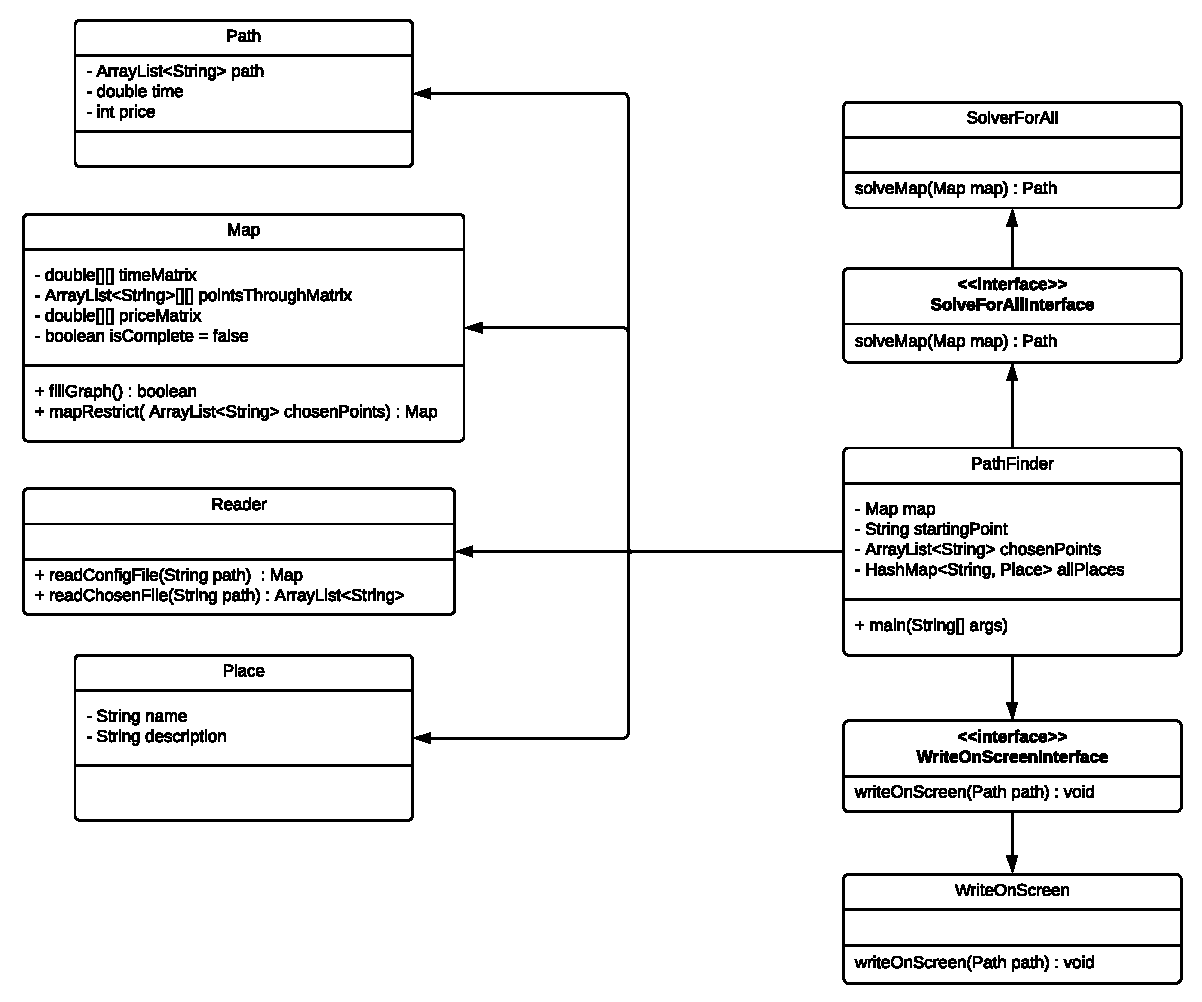
\includegraphics [height=9cm]{diagram_klas.pdf}
\textit{Diagram klas ,,Bieszczadzki Komiwojażer''}
\subsection{Opis klas}
Przedstawienie funkcji i zadań poszczególnych klas.
\subsubsection{PathFinder}

\subsubsection{SolverForAll}

\subsubsection{Path}

\subsubsection{Map}

\subsubsection{Reader}

\subsubsection{Place}

\subsection{Schemat działania}

\section{Struktury danych}
Program będzie wykorzystywał następujące struktury danych.

\subsection{Kopiec}
    Implementacja kolejki priorytetowej
    
\subsection{Macierz}
    Przechowywanie ustrukturyzowanych danych
    
\subsection{HashMap}

\subsection{ArrayList}

\section{Algorytmy}
Podczas rozwiązywania zadanego problemu program będzie korzystał z implementacji następujących algorytmów.

\subsection{Algorytm Djikstry}
Algorytm służy do znajdowania najkrótszej możliwej drogi pomiędzy wybranym wierzchołkiem a pozostałymi wierzchołkami grafu. 

\subsection{Algorytm Helda-Karpa}
Algorytm służy do znajdowania minimalnego drzewa rozpinającego dla grafu pełnego. 

\end{document}